\section{Численные эксперименты}
\subsection{Проверка стабильности имитационной модели}
Для начала проведения численного анализа полученных асимптотических результатов необходимо проверить точность работы реализованной имитационной модели. Для проверки, запустим модель несколько раз с одинаковыми параметрами и для полученных результатов вычислим критерий согласия Колмогорова. Критерий согласия Колмогорова (расстояние Колмогорова) предназначен для проверки гипотезы о том, что некое эмпирическое распределение, в данном случае, распределение, построенное в ходе работы имитационной модели, соответствует предполагаемой модели, которая, в данном случае, так же является результатом работы имитационной модели.

Расстояние Колмогорова вычисляется по следующей формуле
\begin{equation*}
	\Delta = \underset{0 < i < \infty}{max}\bigg\rvert \sum_{v=0}^{i} (P_0(v) - P_1(v))\bigg\rvert.
\end{equation*}

Для численного анализа в данной работе применяется система компьютерной алгебры Mathcad. В ней были построены графики распределения вероятностей и вычислено расстояния Колмогорова для двух запусков имитационной модели с одинаковыми параметрами системы.

Введем следующие обозначения: $\Delta_S$ --- расстояние Колмогорова для суммарного распределения вероятностей, $\Delta_{TD}$ --- расстояние Колмогорова для двумерного распределения. Данные обозначения будут использоваться в дальнейших экспериментах.

\begin{figure}[H]
	\centering
	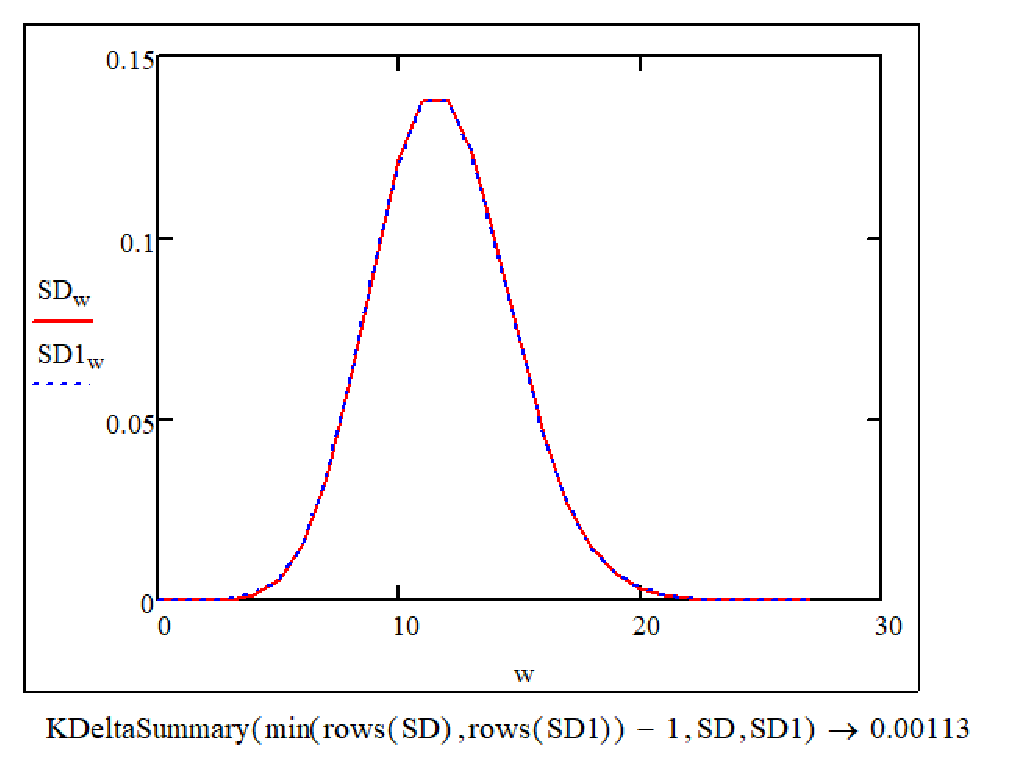
\includegraphics[scale=0.5]{mathcad_check_sim.eps}
	\caption{Сравнение двух отдельных запусков имитационной модели с простейшим входящим потоком}
	\label{experiments_kol_dist_sim}
\end{figure} 

На рисунке \ref{experiments_kol_dist_sim} представлено сравнение двух запусков имитационной модели с параметрами системы: $\lambda = 1, \alpha = 0.5, \sigma = 0.4, \mu_{1} = 6, \mu_{2} = 3, t = 10 $. Запуски модели дали практически одинаковые результаты. Графики рядов распределения вероятностей полностью накладываются друг на друга, а расстояния Колмогорова составили

\begin{equation*}
	\Delta_S = 0.0007,\\
	\Delta_{TD} = 0.0008.
\end{equation*}

Данный эксперимент был проведен и для системы с входящим MMPP--потоком. Были заданы следующие параметры: $\alpha = 0.5, \sigma = 0.4, \mu_{1} = 6, \mu_{2} = 3, t = 10 $,
\begin{equation*}
	\boldsymbol{Q}=\begin{bmatrix}
		-0.3 &  0.1 &  0.2\\
		0.2 & -0.5 &  0.3\\
		0.3 &  0.3 &  -0.6
	\end{bmatrix},
	\boldsymbol{\Lambda}=\begin{bmatrix}
		1 &	0 & 0\\
		0 &	0.6 & 0\\
		0 &	0 & 0.7\\
	\end{bmatrix}.
\end{equation*}

Результаты эксперимента представлены на рисунке \ref{experiments_kol_dist_sim2}

\begin{figure}[H]
	\centering
	\includegraphics[scale=0.5,width=\textwidth]{mathcad_check_sim2.eps}
	\caption{Сравнение двух отдельных запусков имитационной модели с MMPP--потоком}
	\label{experiments_kol_dist_sim2}
\end{figure} 

Графики плотности распределений также полностью накладываются друг на друга, расстояния Колмогорова составили

\begin{equation*}
	\Delta_S = 0.0009,\\
	\Delta_{TD} = 0.0018.
\end{equation*}

Тестирование имитационной модели проводилось с заданным временем моделирования $7\cdot 10^6$. Было выбрано именно такое значение параметра, так как оно дает наивысшую точность, то есть, при установке значение ниже указанного, точность начинает снижаться, а при повышении ее улучшения не наблюдается. Ниже в таблице \ref{time_dynamics} приведена динамика изменения точности запусков модели при одинаковых параметрах в зависимости от заданного времени моделирования. Максимальное время моделирование, которое допускает реализация программы --- $10^7$. Параметры системы соответствуют параметрам из эксперимента на рисунке \ref{experiments_kol_dist_sim}.

\begin{table}[h!] 
	\centering
	\caption{Расстояние Колмогорова при различных значениях параметра времени моделирования}
	\label{time_dynamics}
	\begin{tabular}{| c | c | c | c | c | c |} 
		\hline
		$t$ & $5\cdot 10^4$ & $10^6$ & $5\cdot 10^6$ & $7\cdot 10^6$ & $10^7$\\ 
		\hline
		$\Delta_S$ & 0.011 & 0.0023 & 0.0016 & 0.0007 & 0.0008\\
		\hline
		$\Delta_{TD}$ & 0.0176 & 0.0034 & 0.0022 & 0.0008 & 0.0012\\
		\hline
	\end{tabular}
\end{table} 

Исходя из вышеописанных экспериментов, можно сделать вывод, что реализованная имитационная модель дает стабильные результаты, что подтверждают вычисленные значения расстояния Колмогорова для обоих видов распределений --- его значение не превышает порог в $10^{-3}$. Следовательно, модель может быть применена для анализа и оценки применимости асимптотических результатов с указанной погрешностью.
\subsection{Оценка точности асимптотических результатов}
Теперь, когда стабильность имитационной модели подтверждена экспериментально, сравним результаты ее работы с полученным асимптотическим приближением функции распределения вероятностей числа обслуженных заявок для систем, рассмотренных в разделах \ref{section_simple_summary}, \ref{section_simple_twodim} и \ref{section_map_twodim} при разной интенсивности возврата заявок с орбиты. Значение этого параметра влияет на точность при сравнении, так как решение систем было получено при асимптотическом условии большой задержки заявок на орбите.

Для того, чтобы проиллюстрировать влияние задержки заявок на орбите на получаемый результат для RQ--системы с простейшим входящим потоком, зададим ее параметры:
\begin{equation} \label{simple_summary_input_params}
	\lambda = 2,
	\alpha = 0.9,
	\mu_{1} = 3.5,
	\mu_{2} = 2.1, 
	t = 15.
\end{equation}
Теперь рассчитаем распределения вероятностей числа обслуженных заявок по формуле \eqref{distr_simple_summary} и сделаем несколько запусков имитационной модели, варьируя интенсивность возращения заявок с орбиты $\sigma$.

\begin{table}[h!] 
	\centering
	\caption{Расстояние Колмогорова при различных значениях параметра $\sigma$}
	\label{table_simple_summary}
	\begin{tabular}{| c | c | c | c | c | c | c | c | c |}
		\hline
		$\sigma$ & 10 & 1 & 0.6 & 0.4 & 0.2 & 0.1 & 0.05 & 0.01 \\ 
		\hline
		$\Delta_S$ & 0.022 & 0.015 & 0.0112 & 0.01 & 0.006 & 0.004 & 0.002 & 0.002\\
		\hline
		$\Delta_{TD}$ & 0.04 & 0.026 & 0.02 & 0.015 & 0.009 & 0.006 & 0.003 & 0.002\\
		\hline
	\end{tabular}
\end{table}

Как видно в таблице \ref{table_simple_summary}, при сравнении работы имитационной модели и асимптотических результатов расстояние Колмогорова тем меньше, чем меньше интенсивность возврата заявок с орбиты. Однако, даже при больших значениях $\sigma$, таких как 10 и 1, мы получаем результаты, где расстояние Колмогорова составляет не больше четырех сотых. В нижней строчке таблицы \ref{table_simple_summary} представлены расчеты для двумерного распределения вероятности числа обслуженных заявок. Можно видеть, что в случае двумерного распределения расстояние Колмогорова значительно больше при больших значениях $\sigma$, однако оно сходится к такому же значению при $\sigma = 0.01$, что и в случае одномерного распределения.

Чтобы проверить, наблюдается ли подобная тенденция при большей загруженности системы, установим в ранее описанных параметрах \eqref{simple_summary_input_params} $\lambda = 2.7$. Тогда получим следующий результат

\begin{table}[h!] 
	\centering
	\caption{Расстояние Колмогорова при различных значениях параметра $\sigma$ при повышенной интенсивности прихода заявок}
	\label{table_simple_summary_high_lambda}
	\begin{tabular}{| c | c | c | c | c | c | c | c | c |}
		\hline
		$\sigma$ & 10 & 1 & 0.6 & 0.4 & 0.2 & 0.1 & 0.05 & 0.01 \\ 
		\hline
		$\Delta_S$ & 0.007 & 0.004 & 0.004 & 0.003 & 0.003 & 0.003 & 0.001 & 0.001\\
		\hline
		$\Delta_{TD}$ & 0.02 & 0.01 & 0.007 & 0.004 & 0.003 & 0.002 & 0.002 & 0.001\\
		\hline
	\end{tabular}
\end{table}

Как видно в таблице \ref{table_simple_summary_high_lambda}  при повышенной загруженности системы также наблюдается тенденция к уменьшению расстояния Колмогорова, однако, асимптотические результаты оказываются значительно точнее.

Поскольку интенсивность вызова прибором заявок также влияет на количество заявок на орбите, проведем расчеты с параметрами \eqref{simple_summary_input_params}, установив $\alpha = 1.6$.

\begin{table}[h!] 
	\centering
	\caption{Расстояние Колмогорова при различных значениях параметра $\sigma$ при повышенной интенсивности вызова заявок}
	\label{table_simple_summary_high_alpha}
	\begin{tabular}{| c | c | c | c | c | c | c | c | c |}
		\hline
		$\sigma$ & 10 & 1 & 0.6 & 0.4 & 0.2 & 0.1 & 0.05 & 0.01 \\ 
		\hline
		$\Delta_S$ & 0.007 & 0.006 & 0.005 & 0.005 & 0.005 & 0.002 & 0.001 & 0.002\\
		\hline
		$\Delta_{TD}$ & 0.024 & 0.015 & 0.011 & 0.01 & 0.007 & 0.003 & 0.002 & 0.001\\
		\hline
	\end{tabular}
\end{table}

Из расчетов в таблице \ref{table_simple_summary_high_alpha} видно, что также при увеличении задержки заявок на орбите, асимптотические результаты становятся точнее, однако в целом их точность снижается.

Для проведения данного эксперимента с RQ--системой, где в качестве источника заявок выступает MMPP--поток, зададим следующие параметры:
\begin{equation*} \label{map_summary_input_params}
	\alpha = 0.6,
	\mu_{1} = 2,
	\mu_{2} = 1.5, 
	t = 15,
\end{equation*}
 \begin{equation*}
 	\boldsymbol{Q}=\begin{bmatrix}
 		-0.5 &  0.2 &  0.3\\
 		0.15 & -0.2 &  0.05\\
 		0.3 &  0.4 &  -0.7
 	\end{bmatrix},
 	\boldsymbol{\Lambda}=\begin{bmatrix}
 		1 &	0 & 0\\
 		0 &	0.6 & 0\\
 		0 &	0 & 0.7\\
 	\end{bmatrix}.
 \end{equation*}
\\
Для наглядности, представим интенсивность входящего потока как $r\cdot\Lambda\cdot E$, в таком случае интенсивность входящего потока составит 0.72. Для указанных параметров системы были получены следующие результаты
\begin{table}[h!] 
	\centering
	\caption{Расстояние Колмогорова при различных значениях параметра $\sigma$ при моделировании MMPP-потока}
	\label{table_map_summary}
	\begin{tabular}{| c | c | c | c | c | c | c | c | c |}
		\hline
		$\sigma$ & 10 & 1 & 0.6 & 0.4 & 0.2 & 0.1 & 0.05 & 0.01 \\ 
		\hline
		$\Delta_S$ & 0.053 & 0.045 & 0.04 & 0.036 & 0.028 & 0.023 & 0.018 & 0.016\\
		\hline
		$\Delta_{TD}$ & 0.059 & 0.049 & 0.042 & 0.035 & 0.024 & 0.015 & 0.01 & 0.003\\
		\hline
	\end{tabular}
\end{table}

Ввиду того, что MMPP--поток труднее поддается моделированию, расстояние Колмогорова для расчетов с ним в среднем больше, однако при маленьких значениях $\sigma$ точность значительно увеличивается. Также, на таблице \ref{table_map_summary} можно заметить, что при меньших $\sigma$ для двумерного распределения асимптотические результаты оказываются точнее.

Повысим загруженность системы, задав новую матрицу интенсивностей с увеличенными значениями диагональных элементов 
 \begin{equation*}
	\boldsymbol{\Lambda}=\begin{bmatrix}
		1.2 &	0 & 0\\
		0 &	0.9 & 0\\
		0 &	0 & 1.5\\
	\end{bmatrix}.
\end{equation*}
Для данных параметров интенсивность потока составит 1.07. Проведем эксперимент с новыми параметрами и получим
\clearpage
\begin{table}[htb!] 
	\centering
	\caption{Расстояние Колмогорова при различных значениях параметра $\sigma$ при повышенной интенсивности вызова заявок}
	\label{table_map_summary_high_lambda}
	\begin{tabular}{| c | c | c | c | c | c | c | c | c |}
		\hline
		$\sigma$ & 10 & 1 & 0.6 & 0.4 & 0.2 & 0.1 & 0.05 & 0.01 \\ 
		\hline
		$\Delta_S$ & 0.037 & 0.029 & 0.024 & 0.02 & 0.015 & 0.01 & 0.008 & 0.008\\
		\hline
		$\Delta_{TD}$ & 0.066 & 0.048 & 0.039 & 0.031 & 0.019 & 0.01 & 0.006 & 0.002\\
		\hline
	\end{tabular}
\end{table}

На основании проведенных экспериментов можно сделать вывод, что тенденция к увеличению точности асимптотических результатов всегда наблюдается при уменьшении значения $\sigma$. При  значении $\sigma$, превышающем интенсивность входящего потока точность не превышает 0.066 (наибольше расстояние Колмогорова, которое наблюдается в случае двумерного распределения вероятностей для системы с MMPP), что говорит о высокой степени точности полученной апрроксимации. Также, повышение загруженности системы заявками входящего потока, как это видно в таблицах \ref{table_simple_summary}, \ref{table_simple_summary_high_lambda} и \ref{table_map_summary}, \ref{table_map_summary_high_lambda}, положительно влияют на точность асимптотических результатов, в то время как увеличение интенсивности вызова заявок прибором делают результаты менее закономерными. Это объясняется тем, что при моделировании в случае повышенной загруженности в системе наступает больше событий за фиксированное время, чем при более низкой.

\subsection{Анализ корреляции выходящих процессов}
В данном разделе проводится анализ корреляции компонентов двумерного выходящего потока рассматриваемого узла обработки запросов.

Для того, чтобы проиллюстрировать изменение корреляции, был проведен ряд экспериментов с вариацией изначальных параметров.
Для RQ--системы с простейшим входящим потоком зададим следующими исходные параметры:
\begin{equation} \label{simple_summary_input_params_corr}
	\lambda = 1,
	\alpha = 1,
	\mu_{1} = 20,
	\mu_{2} = 20, 
	t = 10.
\end{equation}

Поскольку, корреляция может изменяться под влиянием различных параметров, будем варьировать пары выбранных параметров в определенном диапазоне. В первую очередь проведем расчеты корреляции при изменяющихся интенсивностях обслуживания входящих и вызываемых заявок с помощью формул, полученных в разделе \ref{corr_section}. Диапазон: $\mu_{1},\mu_{2} \in [2,16]$

\begin{figure}[H]
	\centering
	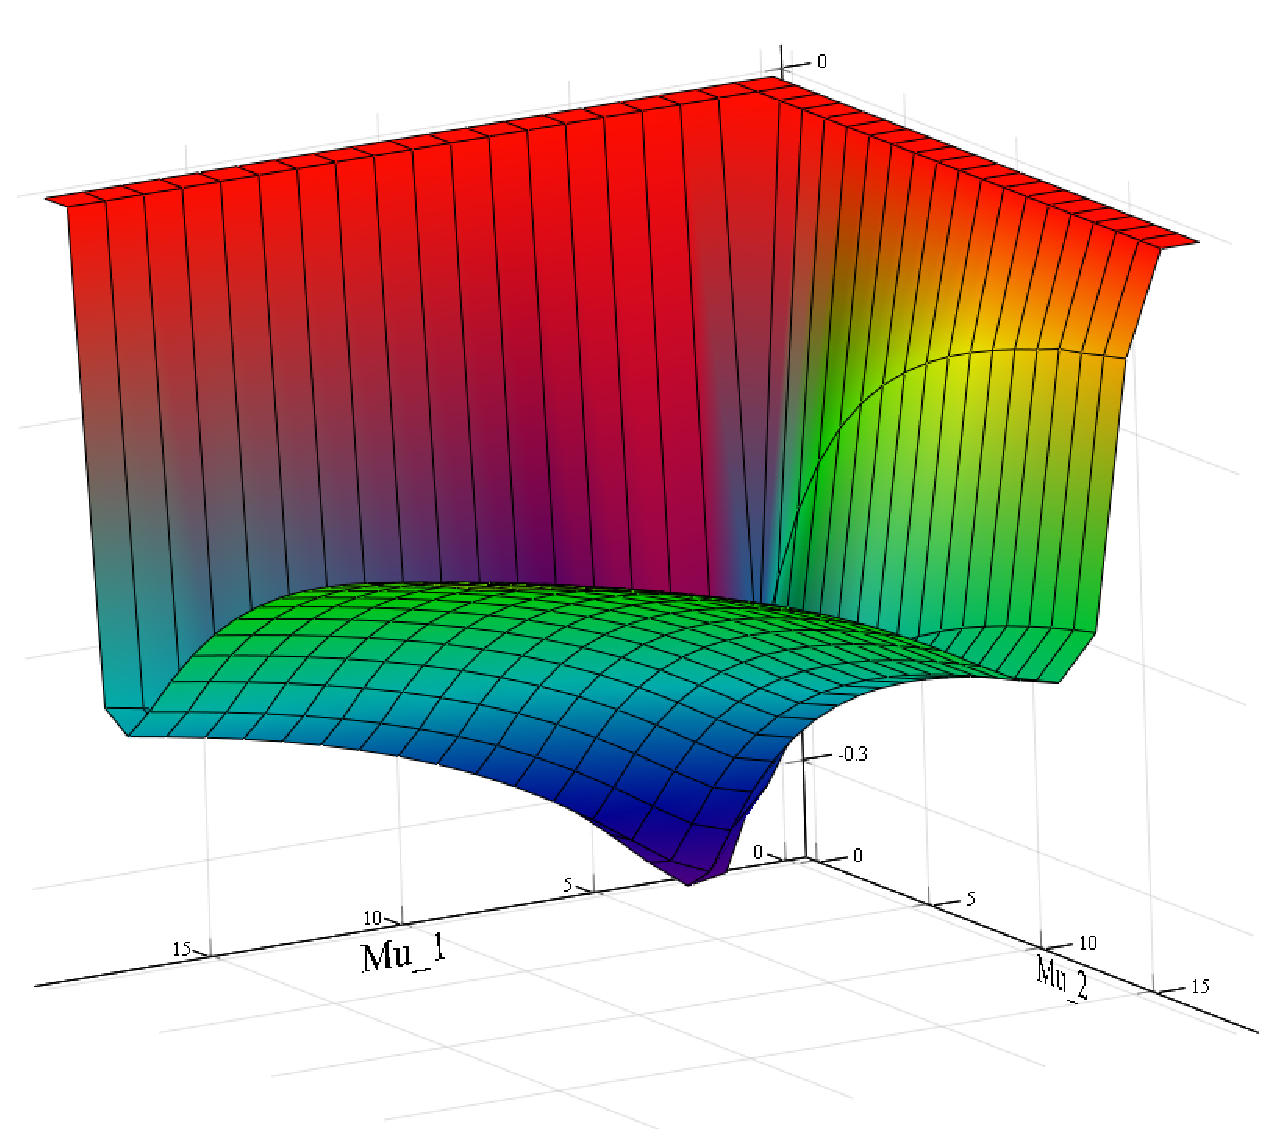
\includegraphics[scale=0.5]{corr_exp1.eps}
	\caption{Изменение корреляции при различных интенсивностях обслуживания}
	\label{exps_corr_exp1}
\end{figure} 

На рисунке \ref{exps_corr_exp1} представлено изменение коэффициента корреляции компонентов выходящего потока при варьировании $\mu_{1}$ и $\mu_{2}$. Коэффициент в выбранном диапазоне всегда имеет отрицательное значение, что означает снижение количества обслуженных заявок одного типа при увеличении другого. Также можно заметить, что при увеличении $\mu_{1}$ значение коэффициента корреляции ниже, чем при увеличении $\mu_{2}$. Это объясняется тем, что заявки входящего потока рано или поздно получать доступ к ресурсу, а их частое нахождение на приборе уменьшает время для поступления вызываемых заявок, которые при неудачной попытке поступления на прибор теряются.

Возьмем другую пару параметров для вариации: $\alpha,\lambda \in [2,16]$

\begin{figure}[H]
	\centering
	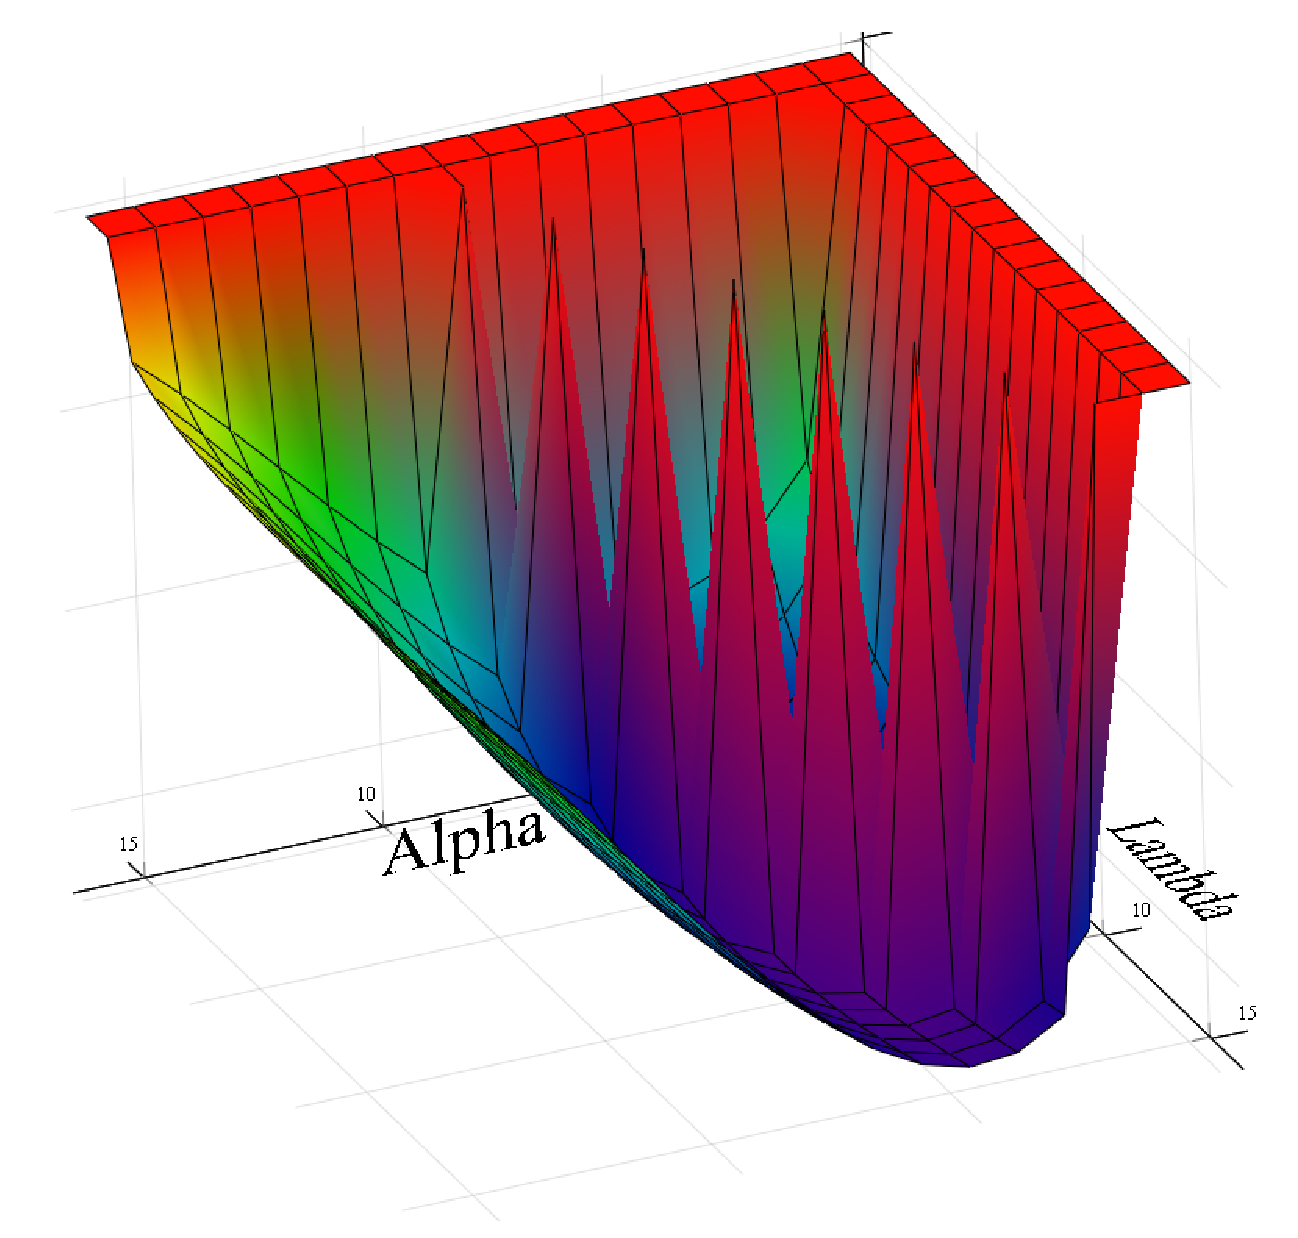
\includegraphics[scale=0.5]{corr_exp2.eps}
	\caption{Изменение корреляции при различных интенсивностях поступления заявок}
	\label{exps_corr_exp2}
\end{figure} 

Для данных параметров по сравнению с варьированием $\mu_{1}$ и $\mu_{2}$ наблюдается обратная тенденция --- при увеличении интенсивности поступления вызываемых заявок корреляция ниже, чем при более интенсивном входящем потоке заявок. Помимо этого, в результате проведенных расчетов были найдены параметры системы, при которых процессы обслуживания входящих заявок и вызываемых становятся независимыми. С данными параметрами с помощью имитационной модели было получено эмпирическое распределение вероятностей, на основе которого также была вычислена корреляция. Результаты совпадают, однако для подробного объяснения нулевого значения коэффициента корреляции при указанных параметрах требуется дальнейшее исследование в этом направлении.
Также стоит отметить, что при увеличении интенсивности входящего потока корреляция в целом стремится к нулю.

Расчеты для параметров: $\mu_{2},\lambda \in [2,16]$ и $\mu_{1},\alpha \in [2,16]$
\begin{figure}[H]
	\centering
	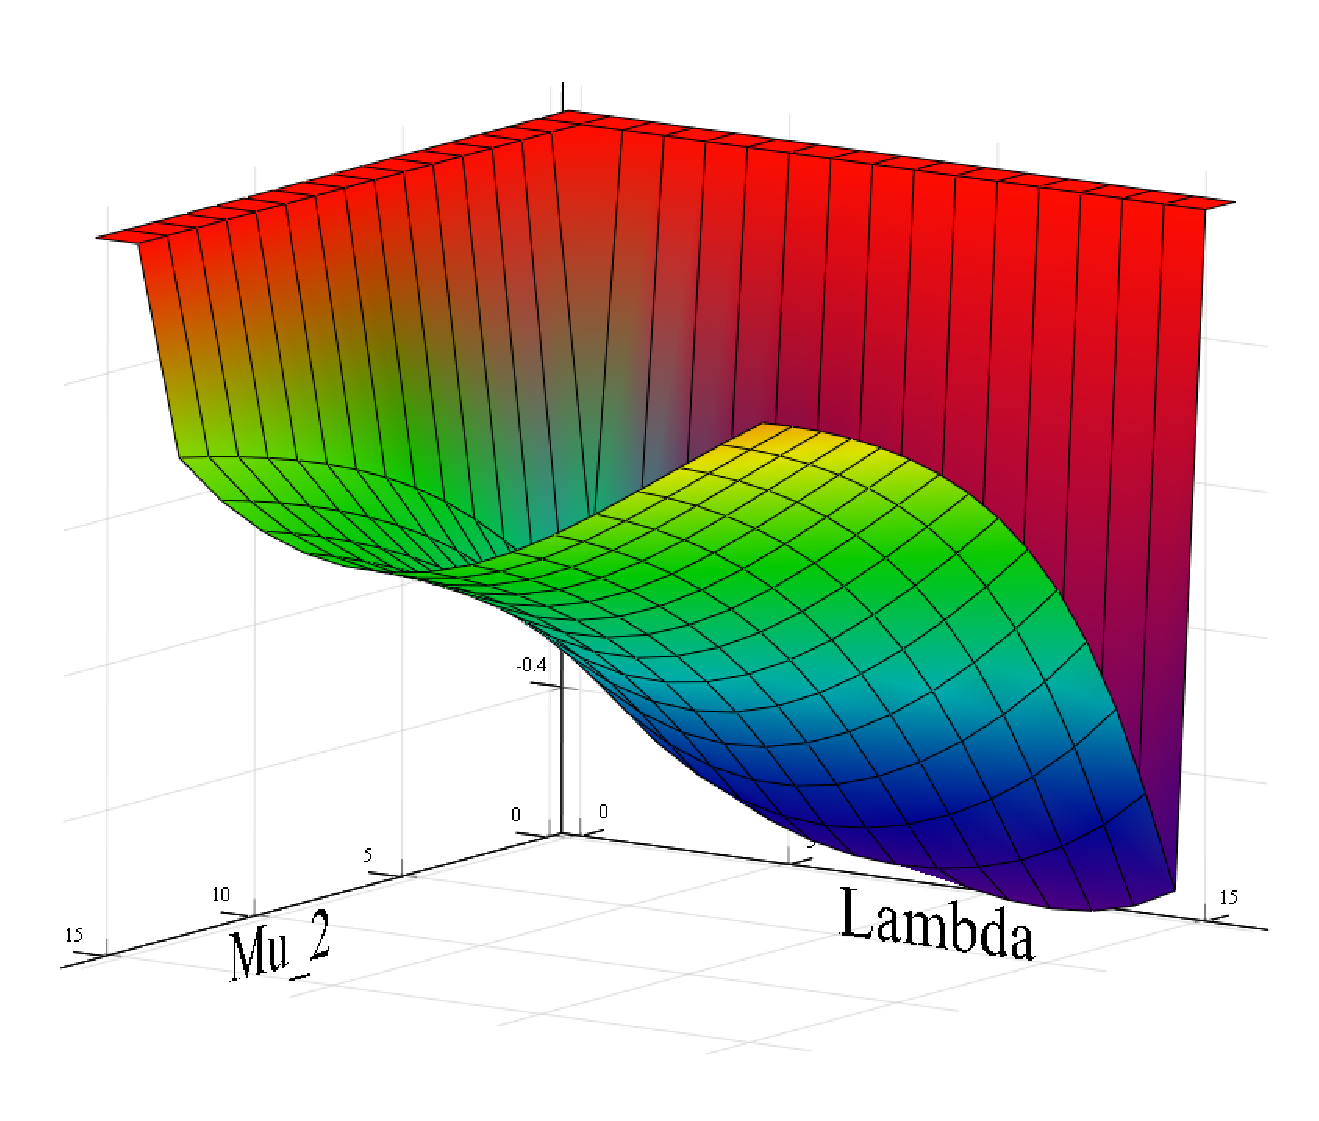
\includegraphics[scale=0.5]{corr_exp3.eps}
	\caption{Изменение корреляции при различных интенсивности обслуживания вызванных и интенсивности поступления заявок}
	\label{exps_corr_exp3}
\end{figure} 

\begin{figure}[H]
	\centering
	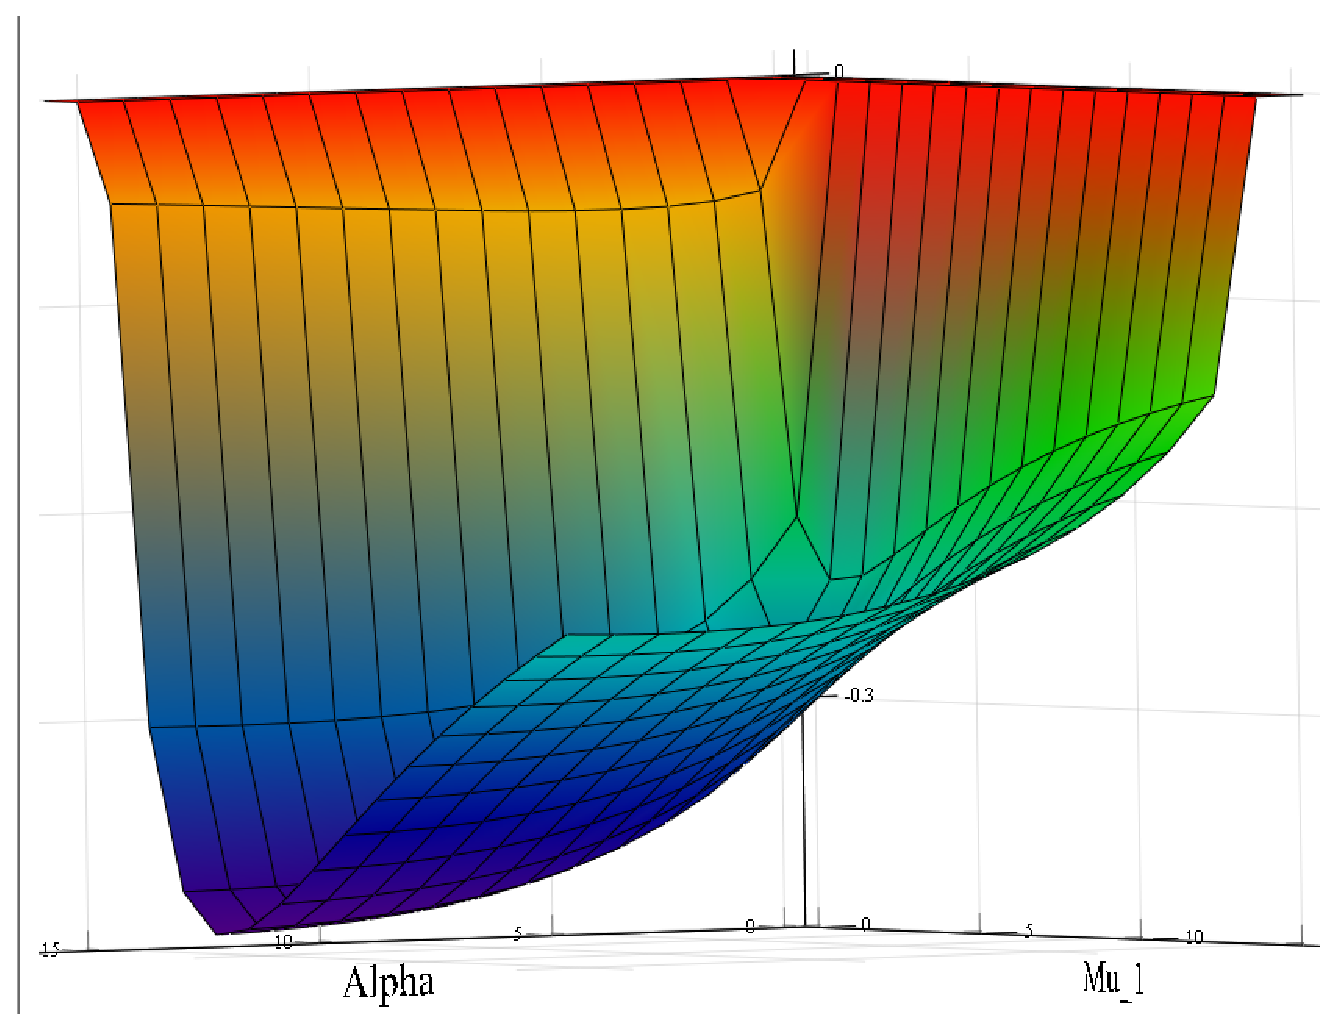
\includegraphics[scale=0.5]{corr_exp5.eps}
	\caption{Изменение корреляции при различных интенсивности обслуживания входящих и интенсивности вызова заявок}
	\label{exps_corr_exp5}
\end{figure} 

На рисунках \ref{exps_corr_exp3} и \ref{exps_corr_exp5} представлены расчеты коэффициента корреляции для интенсивностей поступления в систему одного типа заявок и интенсивности обслуживания другого. Расчеты представлена вместе, так как в них наблюдается закономерность --- при увеличении интенсивности поступления коэффициент корреляции принимает меньшие значения, а также он всегда отрицательный.

Теперь проведем расчеты для пар параметров одного типа заявок: $\mu_{2},\alpha \in [2,16]$ и $\mu_{1},\lambda \in [2,16]$
\begin{figure}[H]
	\centering
	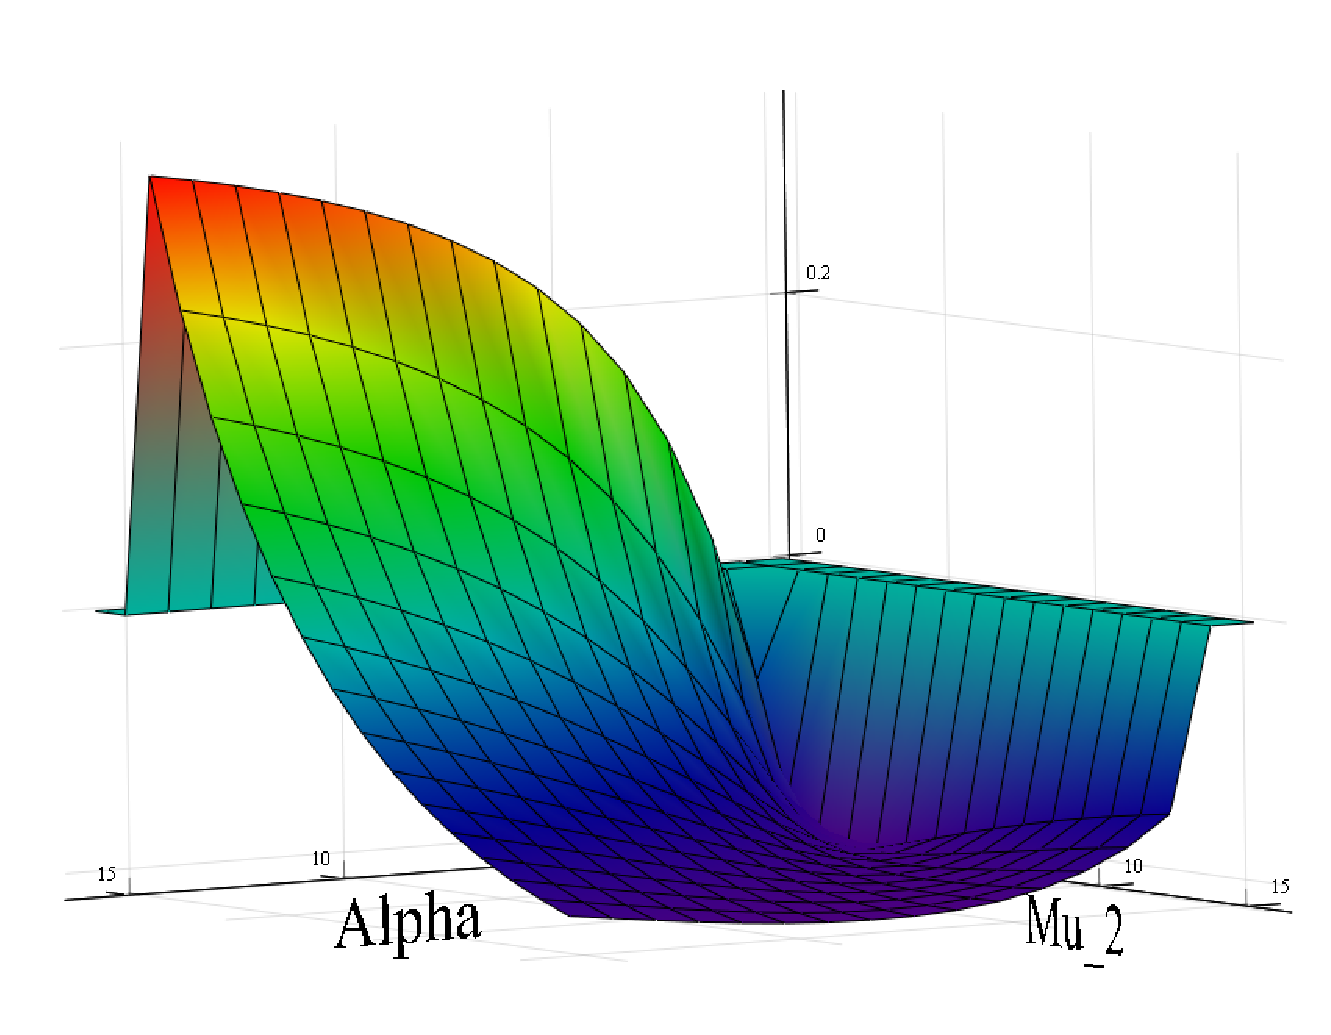
\includegraphics[scale=0.5]{corr_exp4.eps}
	\caption{Изменение корреляции при различных интенсивности обслуживания вызванных и интенсивности вызова заявок}
	\label{exps_corr_exp4}
\end{figure} 

\begin{figure}[H]
	\centering
	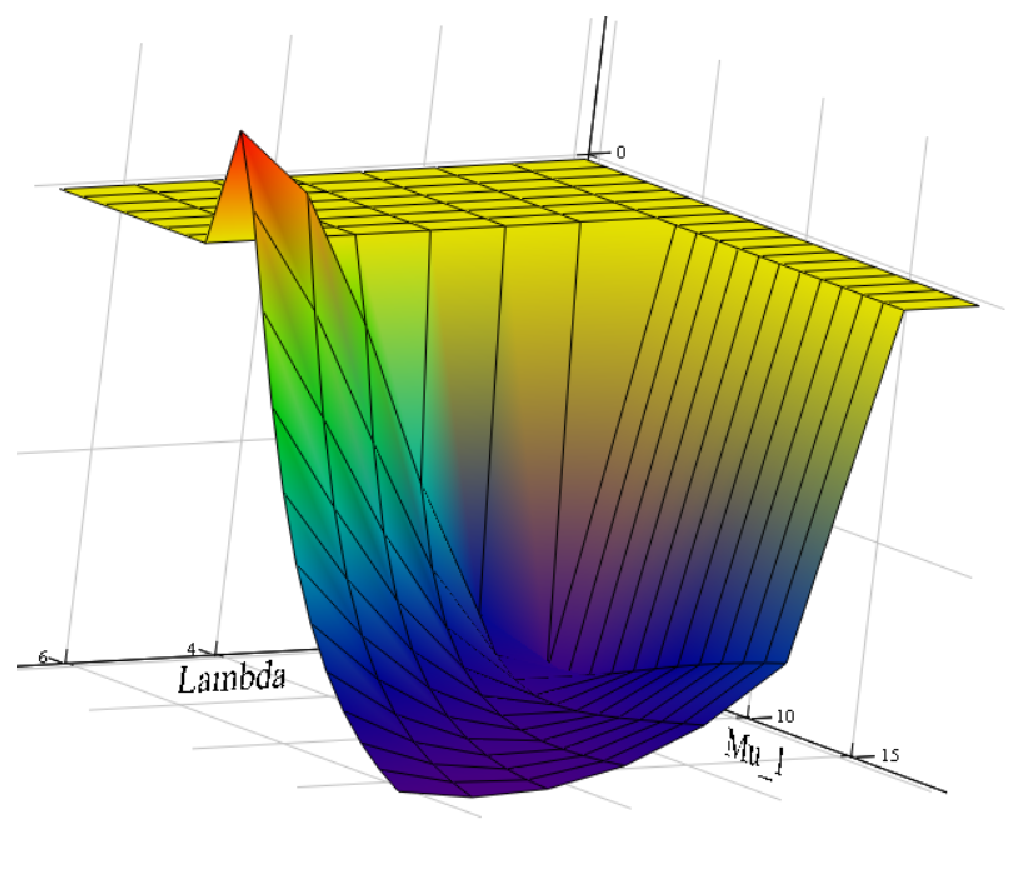
\includegraphics[scale=0.5]{corr_exp6.eps}
	\caption{Изменение корреляции при различных интенсивностях входящего потока и интенсивности обслуживания входящих заявок}
	\label{exps_corr_exp6}
\end{figure} 

При варьировании указанных наборов параметров на рисунках \ref{exps_corr_exp4} и \ref{exps_corr_exp6} видно, что коэффициент корреляции принимает как положительные, так и отрицательные значения.

Для RQ--системы с MMPP формула из раздела \ref{corr_section} не дает интерпретируемых результатов, поэтому для нее коэффициент корреляции был вычислен точечно при помощи распределения вероятностей, полученного в результаты имитационного моделирования при параметрах MMPP, соответствующих интенсивности простейшего входящего потока. Для этого были заданы следующие параметры системы:
 \begin{equation} \label{mmpp_corr_test_params}
\mu_{1},\mu_{2} \in (2,4,6,8), \alpha = 0.8,\sigma = 0.1, t = 15,
\end{equation}
 \begin{equation*}
	\boldsymbol{\Lambda}=\begin{bmatrix}
		0.94 &	0 & 0\\
		0 &	1.25 & 0\\
		0 &	0 & 1.56\\
	\end{bmatrix},
\boldsymbol{Q}=\begin{bmatrix}
	-0.2 &	0.1 & 0.1\\
	0.3 &	-0.5 & 0.2\\
	0.2 & 0.4 & -0.6\\
\end{bmatrix}.
\end{equation*}

При данной матрице $\Lambda$ общая интенсивность MMPP, вычисляемая, как $r\cdot Q\cdot E$ равна 1.13. Соответствующая интенсивность была задана для простейшего потока входящих заявок.

\begin{table}[htb!] 
	\centering
	\caption{Расчеты коэффициента корреляции для RQ--системы с MMPP}
	\label{corr_mmpp_table}
	\begin{tabular}{| c | c | c | c | c || c | c | c | c | c |}
		\hline
		$\mu_{2}$/$\mu_{1}$ & 2 & 4 & 6 & 8 & $\mu_{2}$/$\mu_{1}$ &  2 & 4 & 6 & 8\\ 
		\hline
		2 & -0.217 & -0.347 & -0.327 & -0.297 & 2 & -0.21 & -0.346 & -0.329 & -0.307 \\
		\hline
		4 & -0.126 & -0.289 & -0.278 & -0.256 & 4 & -0.114 & -0.288 & -0.282 & -0.264 \\
		\hline
		6 & -0.079 & -0.246 & -0.237 & -0.22 & 6 & -0.067 & -0.244 & -0.24 & -0.223\\
		\hline
		8 & -0.057 & -0.224 & -0.211 & -0.196 & 8 & -0.041 & -0.216 & -0.212 & -0.197\\
		\hline
	\end{tabular}
\end{table}

В таблице \ref{corr_mmpp_table} показаны результаты вычисления коэффициента корреляции для RQ--системы с MMPP--потоком с параметрами \eqref{mmpp_corr_test_params} при помощи имитационного моделирования (слева) и результаты вычисления коэффициента корреляции для системы c теми же параметрами с простейшим входящим потоком, графическое представление которых представлено на рисунке \ref{exps_corr_exp1} (cправа), при том условии, что интенсивности входящих потоков равны. Корреляция для системы с MMPP ввиду распределения вероятностей, полученного при моделировании, была вычислена с некоторой погрешностью, однако для соответствующих значений $\mu_{1}$ и $\mu_{2}$ коэффициенты приблизительно равны.
\clearpage
